\documentclass{standalone}
\usepackage[T1]{fontenc}
\usepackage[utf8]{inputenc}
\usepackage{pgf,tikz}
\usepackage{setspace}
\usepackage{pgfplots}
\pgfplotsset{compat=1.13}
\usepackage{romannum}

\usepgfplotslibrary{groupplots}

\begin{document}



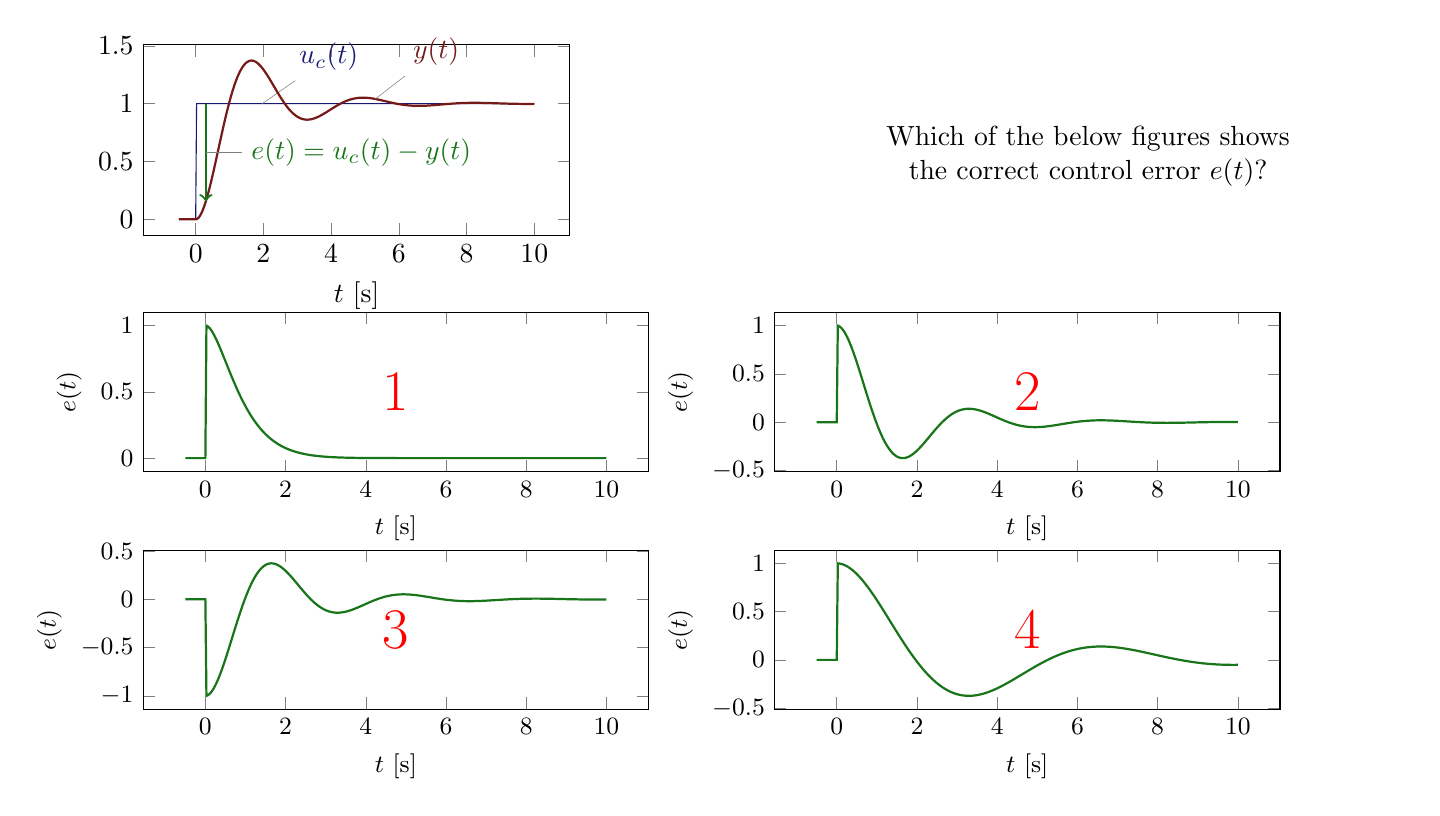
\begin{tikzpicture}

\pgfmathsetmacro{\ww}{2}
\pgfmathsetmacro{\zz}{0.3}

\begin{axis}[
  clip=false,
  yshift=3cm,
  height=4cm,
  width=7cm,
  %axis lines=middle, 
  %xmin=-1, xmax=1,
  %ymin=-2, ymax=2,
  xlabel={$t$ [s]},
  ylabel={},
  %xtick=\empty,
  %ytick = {-1, 1},
  %yticklabels = {$-i\frac{\pi}{4}$, $-i\frac{\pi}{4}$},
  %title={s-plane}
]
\addplot+[black!60!blue!90, no marks, domain=-0.5:10, samples=400] {(x>0)} node [pos=0.3,  coordinate, pin=40:{$u_c(t)$}] {};
\addplot+[black!60!red!90, thick, no marks, domain=-0.5:10, samples=400] {(x>0)*(1 - exp(-\ww*\zz*x) / sqrt(1-\zz * \zz) * sin(deg(\ww*sqrt(1 - \zz * \zz)*x) + acos(\zz)))} node [pos=0.58,  coordinate, pin=40:{$y(t)$}] {};

\pgfmathsetmacro{\xx}{0.3}
\pgfmathsetmacro{\yatx}{1 - exp(-\ww*\zz*\xx) / sqrt(1-\zz * \zz) * sin(deg(\ww*sqrt(1 - \zz * \zz)*\xx) + acos(\zz))}

\draw[thick, ->, black!60!green!90] (axis cs: \xx, 1) to  (axis cs: \xx,  \yatx);
\draw[thin, black!60!green!90] (axis cs: \xx, 1) --  (axis cs: \xx,  \yatx) node[pos=0.5, coordinate, pin=0:{$e(t)=u_c(t)-y(t)$}] {};
\end{axis}

\node[align=center, text width=8cm] at (12,4) {Which of the below figures shows the correct control error $e(t)$?};

\pgfplotsset{unitcircle/.style={black, thin, dashed, no marks}}

\pgfmathsetmacro{\wwone}{2}
\pgfmathsetmacro{\zzone}{0.96}

\pgfmathsetmacro{\wwfour}{1}
\pgfmathsetmacro{\zzfour}{0.3}


\def\axlim{1.5}
\begin{groupplot}[
  group style={group size=2 by 2, horizontal sep=16mm,},
  height=3.6cm,width=8cm,
  /tikz/font=\small,
  %xtick={1},
  %ytick=\empty,
  xlabel={$t$ [s]},
  ylabel={$e(t)$},
  %xmin=-\axlim,
  %xmax=\axlim,
  %ymin=-\axlim,
  %ymax=\axlim,
  %axis lines=middle,
  ]

  \nextgroupplot
  \addplot+[black!60!green!90, thick, no marks, domain=-0.5:10, samples=400] {(x>0)*(1-(1 - exp(-\wwone*\zzone*x) / sqrt(1-\zzone * \zzone) * sin(deg(\wwone*sqrt(1 - \zzone * \zzone)*x) + acos(\zzone)))};

  \nextgroupplot
  \addplot+[black!60!green!90, thick, no marks, domain=-0.5:10, samples=400] {(x>0)*(1-(1 - exp(-\ww*\zz*x) / sqrt(1-\zz * \zz) * sin(deg(\ww*sqrt(1 - \zz * \zz)*x) + acos(\zz)))};

  \nextgroupplot
  \addplot+[black!60!green!90, thick, no marks, domain=-0.5:10, samples=400] {(x>0)*(-1+(1 - exp(-\ww*\zz*x) / sqrt(1-\zz * \zz) * sin(deg(\ww*sqrt(1 - \zz * \zz)*x) + acos(\zz)))};

  \nextgroupplot
  \addplot+[black!60!green!90, thick, no marks, domain=-0.5:10, samples=400] {(x>0)*(1-(1 - exp(-\wwfour*\zzfour*x) / sqrt(1-\zzfour * \zzfour) * sin(deg(\wwfour*sqrt(1 - \zzfour * \zzfour)*x) + acos(\zzfour)))};


  \end{groupplot}

  %\node[red] at (group c1r1.center) {\large \Romannum{1}};
  \node[red] at (group c1r1.center) {\huge 1};
  \node[red] at (group c2r1.center) {\huge 2};
  \node[red] at (group c1r2.center) {\huge 3};
  \node[red] at (group c2r2.center) {\huge 4};


\end{tikzpicture}
\end{document}

